\documentclass[10pt,letterpaper,english]{article}
\usepackage{mathpazo}
\usepackage[hmargin=2cm,vmargin=2cm]{geometry}
\usepackage{graphicx}
\usepackage{marvosym}
\usepackage{subfigure}
\usepackage{amsmath}
\usepackage{multicol}
\usepackage{float}
\usepackage{booktabs}
\usepackage{enumerate}
\usepackage{dingbat}
\usepackage{tikz-timing}[2009/05/15]
\usepackage{amsthm}% http://ctan.org/pkg/amsthm
\renewcommand*\thesection{\arabic{section}.0}
\usepackage{pdfpages}
\usepackage{calc}
\usetikzlibrary{circuits.logic.US,calc, positioning}
\usepackage{tikz-timing}
%\renewcommand{\familydefault}{\sfdefault}
%\usepackage{helvet}
\usepackage{babel}
\usepackage{fancyhdr}
\pagestyle{empty}
\usepackage[compact]{titlesec}
\titlespacing{\section}{0pt}{2ex}{1ex}
\titlespacing{\subsection}{0pt}{2ex}{1ex}
\titlespacing{\subsubsection}{0pt}{0.4ex}{0ex}


  \hyphenpenalty=500000
  \tolerance=1000

% indentsection style, used for sections that aren't already in lists
% that need indentation to the level of all text in the document
\newenvironment{indentsection}[1]{\begin{list}{}%
{\setlength{\leftmargin}{#1}}%
\item[]%
}{\end{list}}

% opposite of above; bump a section back toward the left margin
\newenvironment{unindentsection}[1]{\begin{list}{}%
{\setlength{\leftmargin}{-0.5#1}}%
\item[]%
}{\end{list}}

% format two pieces of text, one left aligned and one right aligned
\newcommand{\headerrow}[2]{\begin{tabular*}{\linewidth}[t]{l@{\extracolsep{\fill}}r}
#1 &
#2 \\
\end{tabular*}}

\thispagestyle{fancy}
\renewcommand{\headrulewidth}{0pt}
\rfoot{HSV, DJS, RDN}    
\cfoot{}
\begin{document}

\textsc{op-amp configurations}\\
\begin{multicols}{2}
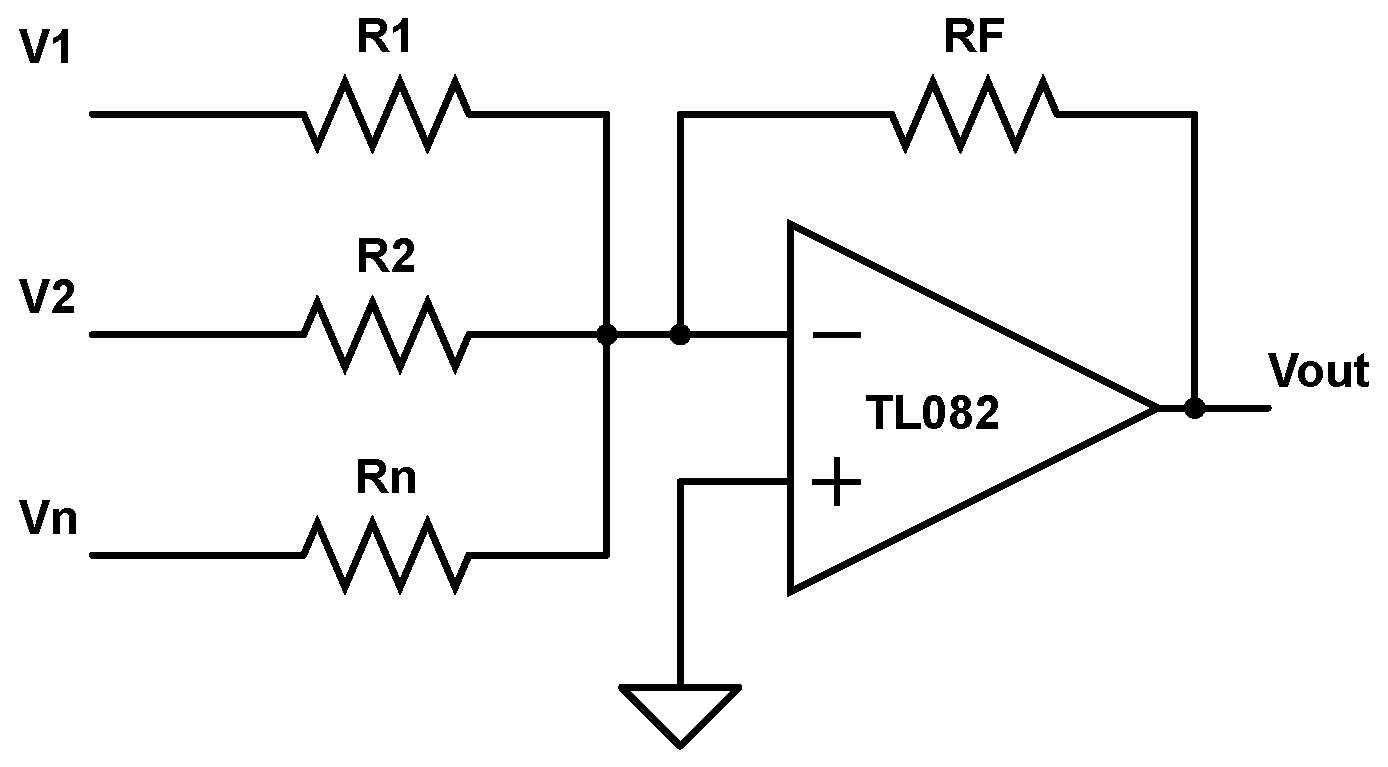
\includegraphics[scale=0.2]{opamp-1.eps}
\begin{align*}
V_{out} = -(\frac{R_F}{R_1}\cdot V_1 + \frac{R_F}{R_2}\cdot V_2 \cdots + \frac{R_F}{R_n}\cdot V_n)
\end{align*}
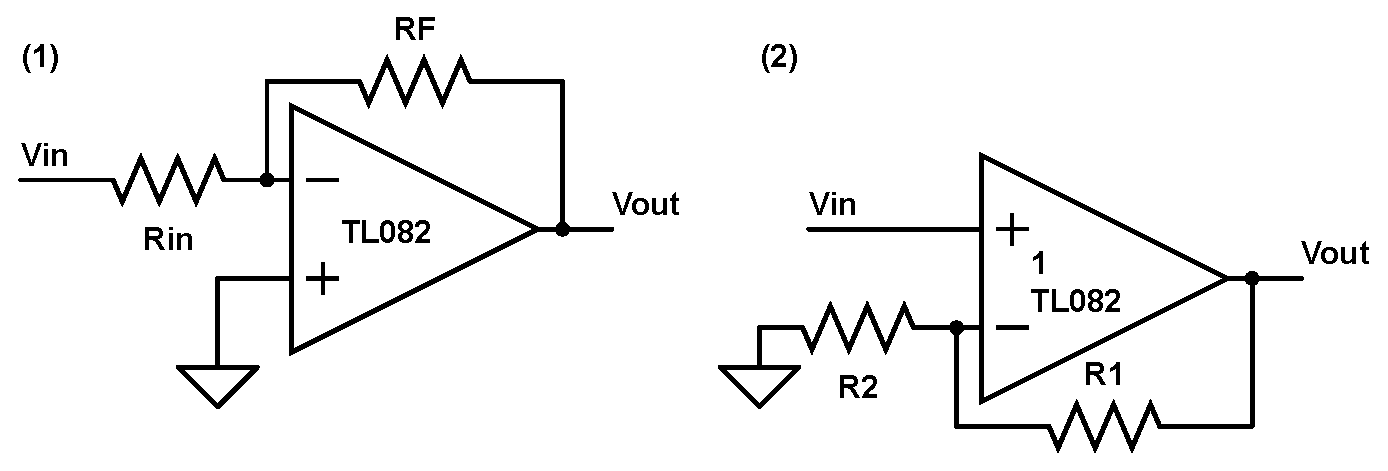
\includegraphics[scale=0.4]{opamp-2.eps}
\begin{align*}
V_{out} = -\frac{R_F}{R_{in}}\cdot V_{in} \tag*{(1) Inverting}\\
V_{out} = (1 + \frac{R_1}{R_2})\cdot V_{in} \tag*{(2) Non-inverting}\\
\end{align*}
\end{multicols}


\begin{multicols}{2}
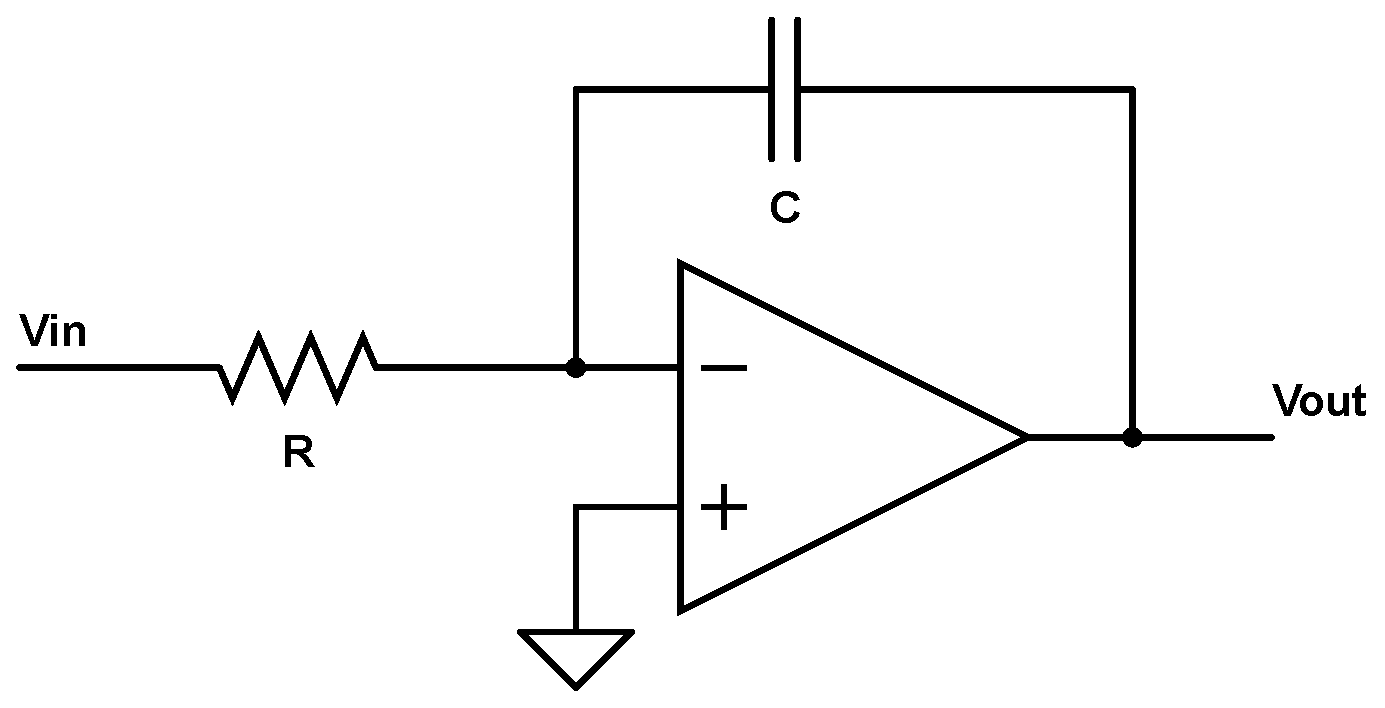
\includegraphics[scale=0.2]{opamp-integrator.eps}
\begin{align*}
V_{out} = -\int_0^t \frac{V_{in}}{RC} \,dt + V_{initial} \tag*{Integrator / Low-pass}\\
\end{align*}
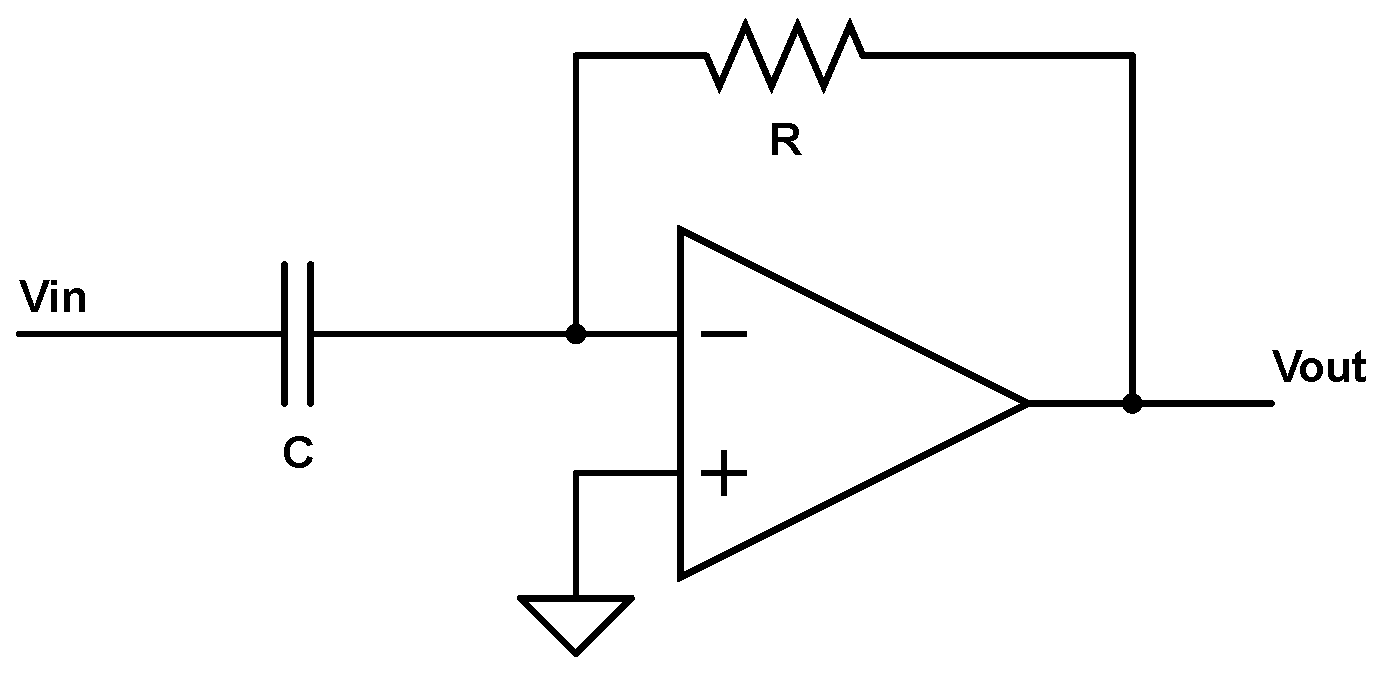
\includegraphics[scale=0.2]{opamp-differentiator.eps}
\begin{align*}
V_{out} = -RC \frac{\,dV_{in}}{\,dt} \tag*{Differentiator / High-pass}\\
\end{align*}
\end{multicols}


\begin{multicols}{2}
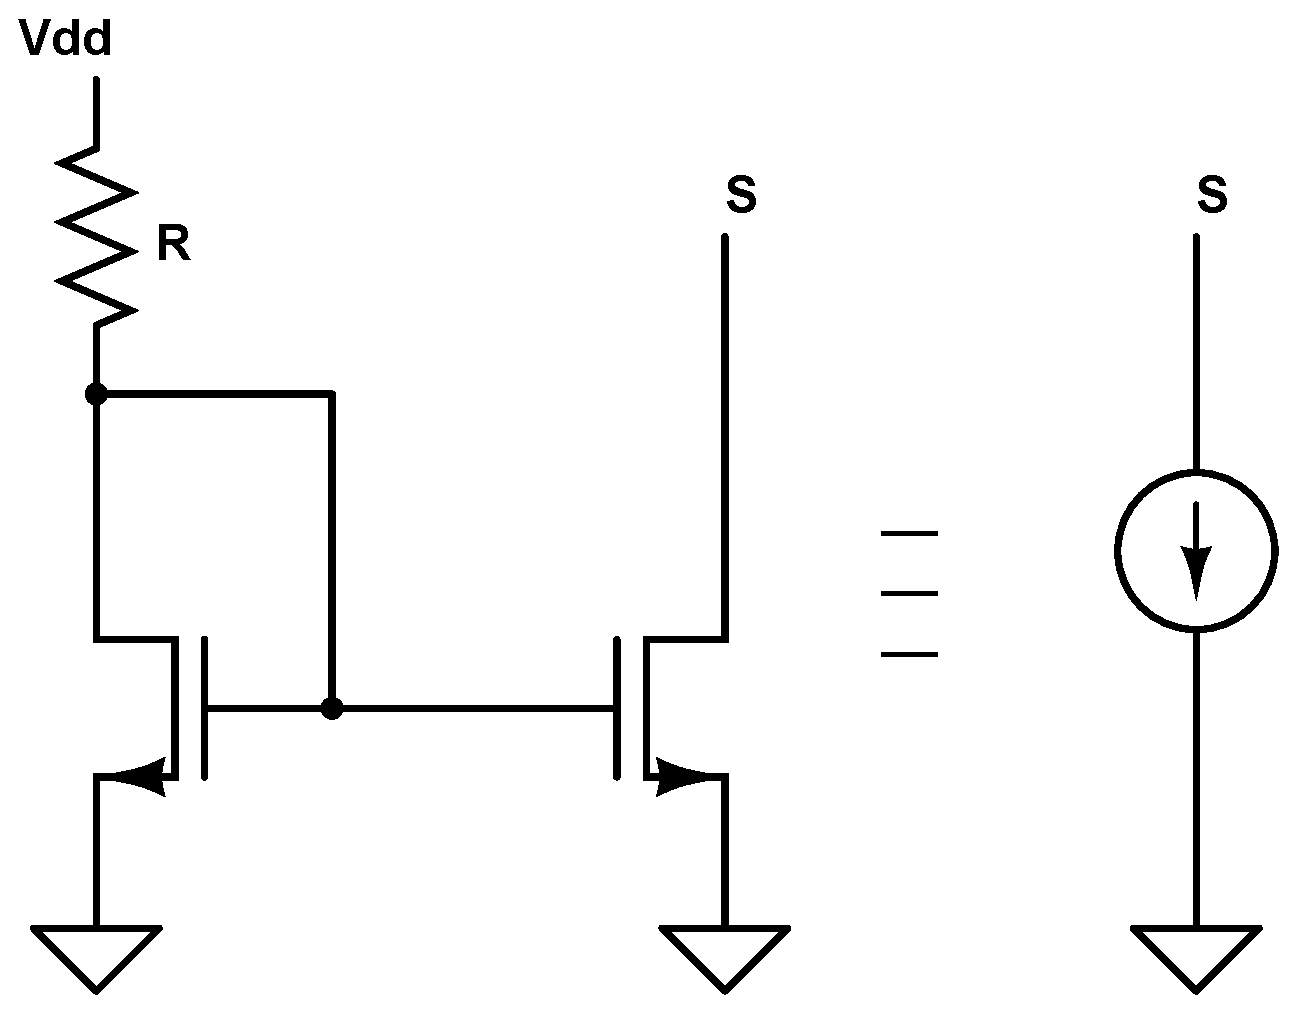
\includegraphics[scale=0.2]{mosfet-current-mirror.eps}
\begin{align*}
\tag*{Mosfet current mirror circuit}\\
\end{align*}
\end{multicols}
\end{document}
